\chapter{La résolution d'équations  du second degré}\label{c.quadratic}

%%%%%%%%%%%%%%%%%%%%%%%%%%%%%%%%%%%%%%%%%%%%%%%%%%%%%%%%%%%%%%%



%%%%%%%%%%%%%%%%%%%%%%%%%%%%%%%%%%%%%%%%%%%%%%%%%%%%%%%%%%%%%%%

Poh-Shen Loh a proposé une méthode de résolution des équations du second degré qui repose sur la  relation entre les coefficients du polynôme et ses racines. La section~\ref{s.traditional} passe en revue les méthodes traditionnelles de résolution des équations du second degré. 
La section~\ref{s.computing} tente de convaincre le lecteur que la méthode de Loh a du sens et explique ensuite comment calculer les racines. Dans la section~\ref{s.examples}, le calcul est effectué pour deux polynômes du second degré et de manière similaire pour un polynôme de degré quatre. La section~\ref{s.general} dérive la formule traditionnelle des racines à partir des formules de Loh.

L'introduction de l'algèbre et de la notation algébrique moderne est relativement récente. Auparavant, les mathématiciens utilisaient presque exclusivement la géométrie. Il est donc intéressant d'examiner la construction géométrique d'Al-Khwârizmî  pour la formule des racines des équations du second degré (sect.~\ref{s.khwar}). La section~\ref{s.cardano} montre une construction géométrique astucieuse utilisée par Cardan pour obtenir la formule des racines des équations de degré trois.

La section~\ref{s.lill-quadratic} présente d'autres méthodes géométriques permettant de trouver les racines d'équations du second degré.\footnote{Le chapitre~\ref{c.origami-cube} est une condition préalable à la compréhension complète de ces méthodes.} Le chapitre se termine par la section~\ref{s.numerical} qui traite du calcul numérique des racines d'équations du second degré.

\section{Méthodes traditionnelles de résolution d'équations du second degré}\label{s.traditional}

Tout étudiant en mathématiques connaît par cœur la formule qui permet d'obtenir les racines d'une équation du second degré $ax^2+bx+c=0$ :
\[
x_1, x_2 = \frac{-b\pm\sqrt{b^2-4ac}}{2a}\,.
\]                      



Pour l'instant nous allons travailler avec des polynômes unitaires, $x^2+bx+c=0$, dont les racines sont 
\begin{align}
x_1, x_2 = \frac{-b\pm\sqrt{b^2-4c}}{2}\,.\label{eq.quadratic-roots}
\end{align}
Une autre méthode de résolution des équations du second degré consiste à factoriser les polynômes plus ou moins par tâtonnement. Il est parfois facile d'obtenir les racines par factorisation :
\begin{align}
x^2-4x+3= (x-1)(x-3)\label{eq.quadratic-lill}\,.
\end{align}
Il est beaucoup plus difficile de factoriser $x^2-2x-24$ car il y a de nombreuses paires de racines possibles qui doivent être prises en compte:
\[
(\pm 1,\mp 24)\,, (\pm 2,\mp 12)\,, (\pm 3,\mp 8)\,, (\pm 4,\mp 6)\,.
\]

\section{La relation entre les racines et les coefficients}\label{s.computing}

\begin{theorem}\label{thm.roots-coefficients}
Si $r_1,r_2$ sont les racines de $x^2+bx+c$ alors 
\[
(x-r_1)(x-r_2)=x^2 - (r_1+r_2)x + r_1r_2=x^2+bx+c\,.
\]
Par conséquent, même si nous ne connaissons pas la valeur des racines, nous savons que
\begin{align}\label{eq.viete-quad}
r_1+r_2 = -b\,,\quad\quad r_1r_2=c\,.
\end{align}
\end{theorem}

Il n'y a vraiment rien à démontrer car le résultat émerge du calcul.

Considérons quelques valeurs de $-b$, $r_1$ et $r_2$, et notons  $m_{12}$  la moyenne de $r_1$ et $r_2$ :
\[
\renewcommand{\arraystretch}{1.2}
\begin{array}{|@{\hspace{1em}}r|@{\hspace{1em}}r|@{\hspace{1em}}r|@{\hspace{1em}}r|}
\hline
-b& r_1 & r_2 &m_{12}\\\hline
33 & 12 & 21 & 16\frac{1}{2}\\\hline
33 & 8 & 25 & 16\frac{1}{2}\\\hline
33 & 1 & 32 & 16\frac{1}{2}\\\hline\hline
-b& r_1 & r_2 &m_{12}\\\hline
-4 & -16 & 12 & -2 \\\hline
-4 & -4 & 0 & -2 \\\hline
-4 & -3 & -1 & -2 \\\hline
\end{array}
\]

Pour toute équation du second degré, la moyenne des deux racines est constante :
\[
m_{1,2}=\frac{r_1+r_2}{2}=
\frac{(-b-r_2)+r_2}{2}=
-\frac{b}{2}\,.
\]



Soit $s$ un nombre quelconque. Alors 
\[
-b=-b+s+(-s)=\left(\frac{-b}{2}+s\right) + \left(\frac{-b}{2}-s\right)=r_1+r_2\,.
\]
Si une racine est à la distance $s$ de la moyenne, l'autre racine est à la distance $-s$ de la moyenne. Pour $r_1=2$ et $r_2=6$, qui correspondent à $m_{12}=4$ et $s=2$, on a :
\[
\renewcommand{\arraystretch}{1.2}
\begin{array}{|@{\hspace{1em}}r|@{\hspace{1em}}r|@{\hspace{1em}}r|@{\hspace{1em}}r|r|r|}
\hline
-b& r_1 & r_2 & m_{12}& m_{12}\!-\!r_1 & m_{12}\!-\!r_2\\\hline
33 & 12 & 21 & 16\frac{1}{2}&4\frac{1}{2} & -4\frac{1}{2}  \\\hline
33 & 8 & 25 & 16\frac{1}{2}&8\frac{1}{2}&-8\frac{1}{2}\\\hline
33 & 1 & 32 & 16\frac{1}{2}&15\frac{1}{2}&-15\frac{1}{2}\\\hline
\hline
-4 & -16 & 12 & -2 &14& -14\\\hline
-4 & -4 & 0 & -2&2&-2 \\\hline
-4 & -3 & -1 & -2&1&-1 \\\hline
\end{array}
\]
La figure~\ref{f.loh-roots1} visualise cette relation.

\begin{figure}[htbp]
\centering
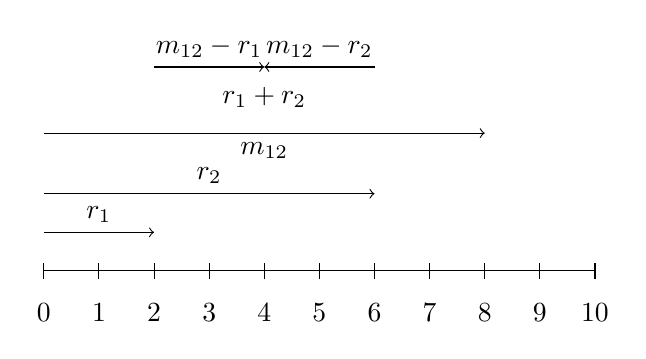
\begin{tikzpicture}[scale=.7]
\begin{scope}[yshift=-4mm]
\draw (0,0) -- (10,0);
\foreach \x in {0,1,...,10}
  \draw (\x,-1.5mm) -- +(0,3mm) node[below,yshift=-4mm] {$\x$};
\draw[->,yshift=7mm] (0,0) -- node[above] {$r_1$} (20mm,0);
\draw[->,yshift=14mm] (0,0) -- node[above] {$r_2$} (60mm,0);
\end{scope}
\draw[->,yshift=21mm] (0,0) -- node[above,yshift=2mm] {$r_1+r_2$} (80mm,0);
\coordinate (M) at (40mm,21mm);
\vertex{M};
\node[below] at (40mm,21mm) {$m_{12}$};
\begin{scope}[yshift=3mm]
\draw[->,yshift=30mm] (20mm,0mm) -- node[above] {$m_{12}-r_1$} +(20mm,0);
\draw[->,yshift=30mm] (60mm,0mm) -- node[above] {$m_{12}-r_2$} +(-20mm,0);
\end{scope}
\end{tikzpicture}
%\includegraphics[width=0.8\textwidth]{Fig7_1}
\caption{Relation entre les racines $r_1=2$, $r_2=6$ et leur moyenne $m_{12}=4$.}
\label{f.loh-roots1}
\end{figure}
Si nous utilisons d'autres valeurs comme $r_1=3$ et $r_2=5$, pour lesquelles $r_1+r_2=8$, alors $m_{12}=4$ reste le même alors que $s=1$ (fig.~\ref{f.loh-roots2}).

Le décalage $s$ semble être arbitraire dans
\[
r_1=\left(\frac{-b}{2}+s\right)\,,\quad r_2=\left(\frac{-b}{2}-s\right)\,,
\]
%\enlargethispage{\baselineskip}
mais il existe une contrainte supplémentaire $r_1r_2=c$, où $c$ est le terme constant du polynôme.
En multipliant les deux expressions que nous avons obtenues pour $r_1$ et $r_2$, nous pouvons déterminer $s$ et ensuite $r_1$ et $r_2$:
\begin{align*}
c&=\left(-\frac{b}{2} +s\right)\left(-\frac{b}{2} -s\right)=
  \frac{b^2}{4}-s^2\\
s&=\frac{\sqrt{b^2-4c}}{2}\,.
\end{align*}

\begin{figure}[htbp]
\centering
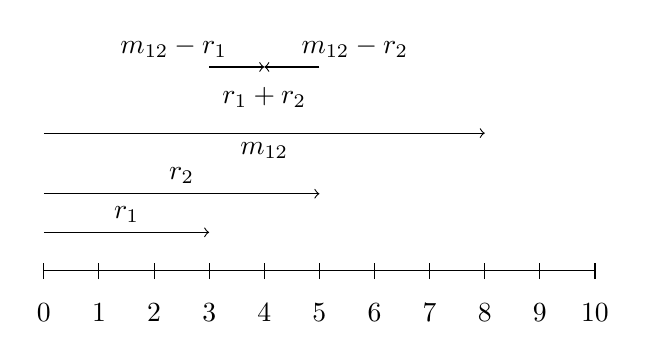
\begin{tikzpicture}[scale=.7]
\begin{scope}[yshift=-4mm]
\draw (0,0) -- (10,0);
\foreach \x in {0,1,...,10}
  \draw (\x,-1.5mm) -- +(0,3mm) node[below,yshift=-4mm] {$\x$};
\draw[->,yshift=7mm] (0,0) -- node[above] {$r_1$} (30mm,0);
\draw[->,yshift=14mm] (0,0) -- node[above] {$r_2$} (50mm,0);
\end{scope}
\draw[->,yshift=21mm] (0,0) -- node[above,yshift=2mm] {$r_1+r_2$}(80mm,0);
\coordinate (M) at (40mm,21mm);
\vertex{M};
\node[below] at (40mm,21mm) {$m_{12}$};
\begin{scope}[yshift=3mm]
\draw[->,yshift=30mm] (30mm,0mm) -- node[above left] {$m_{12}-r_1$} +(10mm,0);
\draw[->,yshift=30mm] (50mm,0mm) -- node[above right] {$m_{12}-r_2$} +(-10mm,0);
\end{scope}
\end{tikzpicture}
%\includegraphics[width=0.8\textwidth]{Fig7_2}
\caption{Relation entre les racines $r_1=3$, $r_2=5$ et leur moyenne $m_{12}=4$.}
\label{f.loh-roots2}
\end{figure}

\section{Exemples de la méthode de Loh}\label{s.examples}

\begin{example}
Considérons le polynôme $x^2-2x-24$ où $b=-2$ et $c=-24$:
\begin{align*}
c&=\left(-\frac{(-2)}{2} +s\right)\left(-\frac{(-2)}{2} -s\right)\\
-24&=(1 +s)(1 -s)\\
%s^2&=&25\\
s&=5\\
r_1&=1+5=6\\
r_2&=1-5=-4\,.
\end{align*}
Vérifions: $(x-6)(x-(-4))= x^2-2x-24$.
\end{example}

\begin{example}
Cherchons les racines de $x^2-83x-2\,310$:
\begin{align*}
%c&=&\left(-\frac{b}{2} +s\right)\left(-\frac{b}{2} -s\right)\\
-2\,310&=\left(\frac{83}{2}+s\right)\left(\frac{83}{2} -s\right)\\
s^2&=\frac{6\,889}{4}+2310=\frac{16\,129}{4}\\
s&=\frac{127}{2}\\
r_1&=\frac{83}{2}-\frac{127}{2}=-22\\
r_2&=\frac{83}{2}+\frac{127}{2}=105\,.
\end{align*}
Vérifions: $(x+22)(x-105)= x^2-83x-2\,310$.



Comparons ce calcul à celui que donne la formule traditionnelle :
\begin{align*}
\frac{-b\pm\sqrt{b^2-4c}}{2}&=\frac{-(-83)\pm\sqrt{(-83)^2-4\cdot (-2\,310)}}{2}\\
%&=& \frac{83\pm\sqrt{6889+9240}}{2} = \frac{83\pm\sqrt{16129}}{2}\\
&= \frac{83\pm\sqrt{16129}}{2} = \frac{83\pm 127}{2}\\
r_1&=\frac{83-127}{2}=-22\\
r_2&=\frac{83+127}{2}=105\,.
\end{align*}
\end{example}

\begin{example}
Le théorème~\ref{thm.roots-coefficients} peut être généralisé aux polynômes de degrés supérieurs. Voici un exemple intéressant pour une équation de degré quatre,  $x^4-10x^2-x+20=0$. Comme pour les équations du second degré, il existe des formules pour résoudre les équations de degré trois et quatre (mais pas les équations de degré supérieur), mais ces formules sont assez compliquées.

Ce polynôme de degré quatre se factorise-t-il en deux polynômes du second degré à coefficients entiers ? Si oui, les coefficients des termes en $x^3$ doivent être égaux et de signes opposés puisque le coefficient du terme en $x^3$ est nul. Par conséquent, la forme des facteurs du second degré est :
\[
f(x) = (x^2 - nx + k_1)\, (x^2 + nx + k_2)\,.
\]
En effectuant la multiplication, on obtient :
\[
\renewcommand{\arraystretch}{1.1}
\begin{array}{rrrrrr}
f(x) = &x^4 & + nx^3 & + k_2 x^2\\
&& -nx^3 &- n^2x^2 &-nk_2x\\
&&&+k_1x^2 &+ nk_1x &+ k_1k_2\,.
\end{array}
\]
En égalant les coefficients, on obtient trois équations pour les trois inconnues $n$, $k_1$ et $k_2$ :
\begin{align*}
(k_1+k_2)-n^2 &= -10\\
n(k_1-k_2) &= -1\\
k_1k_2 &= 20\,.
\end{align*}
Puisque nous cherchons des facteurs avec des coefficients entiers,  il est clair à partir des deux dernières équations que :
\[
n=1,\,k_1=4,\,k_2=5  \quad\quad\textrm{ou} \quad\quad n=1,\,k_1=-5,\, k_2=-4\,.
\]
Seuls $n=1,k_1=-5,\, k_2=-4$ satisfont la première équation pour le coefficient de $x^2$ :
\[
f(x) = (x^2 - x - 5)\, (x^2 + x - 4)\,.
\]



La résolution de ces équations du second degré donne quatre solutions de l'équation de degré quatre :
\[
x = \frac{1\pm\sqrt{21}}{2}  \;\;\textrm{ou} \;\; x= \frac{-1\pm\sqrt{17}}{2} \,.
\]
\end{example}

\section{Obtention de la formule traditionnelle}\label{s.general}

Pour un polynôme unitaire arbitraire $x^2+bx+c$, les formules de Loh sont :
\begin{align*}
c=r_1r_2&=\left(\frac{-b}{2}+s\right)  \left(\frac{-b}{2}-s\right)=\left(\frac{b^2}{4}-s^2\right)\\
s&=\sqrt{\left(\frac{b^2}{4}\right)-c}\\
r_1,r_2&=\frac{-b}{2}\pm\sqrt{\left(\frac{b^2}{4}\right)-c}=\frac{-b\pm\sqrt{b^2-4c}}{2}\,,
\end{align*}
la formule traditionnelle pour obtenir les racines d'un polynôme unitaire du second degré. Si le polynôme n'est pas unitaire, divisons-le par $a$, remplaçons dans l'équation et simplifions :
\begin{align*}
%ax^2+bx+c&=&0\\
x^2+\frac{b}{a}x+\frac{c}{a}&=0\\
r_1,r_2&=\frac{-(b/a)\pm\sqrt{(b/a)^2-4(c/a)}}{2}\\
%&=&\frac{-(b/a)\pm\sqrt{(b/a)^2-4(ac/a^2)}}{2}\\
&=\frac{-b\pm\sqrt{b^2-4ac}}{2a}\,.
\end{align*}

\section{Solution géométrique d'Al-Khwârizmî pour les équations du second degré }\label{s.khwar}

Écrivons un polynôme unitaire du second degré sous la forme $x^2+bx-c$. On peut trouver les racines en complétant le carré :
\begin{align*}
%x^2+bx&=&c\\
x^2+2\left(\frac{b}{2}\right)x+\left(\frac{b}{2}\right)^2&=c+\left(\frac{b}{2}\right)^2\\
\left(x+\frac{b}{2}\right)^2&=c+\left(\frac{b}{2}\right)^2\\
x&=-\frac{b}{2}\pm\sqrt{c+\left(\frac{b}{2}\right)^2}=
\frac{-b\pm\sqrt{b^2+4c}}{2}\,.
\end{align*}
C'est la formule familière pour trouver les racines d'une équation du second degré, sauf que $4c$ a le signe opposé puisque le coefficient du terme constant était $-c$.

La complétion du carré a été développée au VIII$^\text{e}$  siècle par Muhammad ibn Musa al-Khwarizmi dans un contexte géométrique. Étant donné l'équation $x^2+bx=c$, supposons qu'il existe un carré dont le côté est $x$ de sorte que son aire soit  $x^2$.
À l'aire $x^2$, ajoutons $bx$ en ajoutant quatre rectangles d'aire $bx/4$ dont les côtés sont $b/4$ et $x$ (fig.~\ref{f.khw-1}). Complétons maintenant la figure  en un carré en ajoutant les quatre petits carrés d'aire $(b/4)^2$ (fig.~\ref{f.khw-2}).

\vspace{0.4cm}

\begin{minipage}{0.4\textwidth}
\centering      
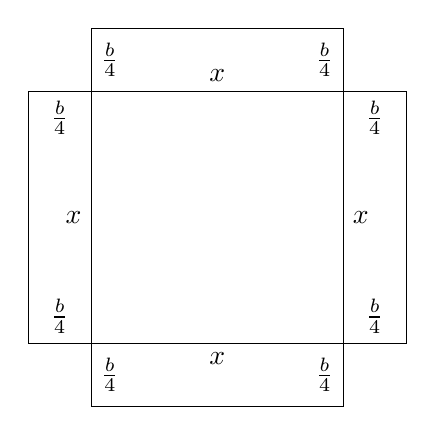
\begin{tikzpicture}[scale=.8]
\coordinate (A) at (0,0);
\coordinate (B) at (4,0);
\coordinate (C) at (4,4);
\coordinate (D) at (0,4);
\draw (A) -- node[below] {$x$} (B) -- node[right] {$x$} (C) -- node[above] {$x$} (D) -- node[left] {$x$} cycle;
\draw (A) -- node[right] {$\frac{b}{4}$} ++(0,-1) -- ++(4,0) -- node[left] {$\frac{b}{4}$} ++(0,1);
\draw (B) -- node[above] {$\frac{b}{4}$} ++(1,0) -- ++(0,4) -- node[below] {$\frac{b}{4}$} ++(-1,0);
\draw (C) -- node[left] {$\frac{b}{4}$} ++(0,1) -- ++(-4,0) -- node[right] {$\frac{b}{4}$} ++(0,-1);
\draw (D) -- node[below] {$\frac{b}{4}$} ++(-1,0) -- ++(0,-4) -- node[above] {$\frac{b}{4}$} ++(1,0);
\end{tikzpicture}
%\includegraphics[width=\textwidth]{Fig7_3a}
         \captionof{figure}{La surface est  $x^2+4(b/4)x=x^2+bx$}
         \label{f.khw-1}  
     \end{minipage}
     \hspace{3em}
     \begin{minipage}{0.4\textwidth}
\centering   
\begin{tikzpicture}[scale=.8]
\coordinate (A) at (0,0);
\coordinate (B) at (4,0);
\coordinate (C) at (4,4);
\coordinate (D) at (0,4);
\draw (A) -- node[below] {$x$} (B) -- node[right] {$x$} (C) -- node[above] {$x$} (D) -- node[left] {$x$} cycle;
\draw (A) -- node[right] {$\frac{b}{4}$} ++(0,-1) -- ++(4,0) -- node[left] {$\frac{b}{4}$} ++(0,1);
\draw (B) -- node[above] {$\frac{b}{4}$} ++(1,0) -- ++(0,4) -- node[below] {$\frac{b}{4}$} ++(-1,0);
\draw (C) -- node[left] {$\frac{b}{4}$} ++(0,1) -- ++(-4,0) -- node[right] {$\frac{b}{4}$} ++(0,-1);
\draw (D) -- node[below] {$\frac{b}{4}$} ++(-1,0) -- ++(0,-4) -- node[above] {$\frac{b}{4}$} ++(1,0);
\draw[thick,dashed] ($(A)+(0,-1)$) -- ++(-1,0) -- ++(0,1);
\draw[thick,dashed] ($(B)+(0,-1)$) -- ++(1,0) -- ++(0,1);
\draw[thick,dashed] ($(C)+(0,1)$) -- ++(1,0) -- ++(0,-1);
\draw[thick,dashed] ($(D)+(0,1)$) -- ++(-1,0) -- ++(0,-1);
\end{tikzpicture}
%\includegraphics[width=\textwidth]{Fig7_3b}
         \captionof{figure}{La surface est 
 $x^2+4(b/4)x+4(b/4)^2=x^2+bx+(b^2/4)$}
         \label{f.khw-2}
     \end{minipage}
     
\vspace{0.4cm}




On ne peut pas construire  la figure~\ref{f.khw-1} car on ne sait pas ce qu'est $x$, mais l'aire du plus grand carré de la figure~\ref{f.khw-2} est 
\[
x^2+bx+\frac{b^2}{4}=c+\frac{b^2}{4}\,,
\]
que nous connaissons puisque les coefficients $b$ et $c$  sont donnés. En construisant la figure  et en effaçant les petits carrés dont les côtés sont $(b/4)$ --- une autre quantité connue --- on obtient le segment  de longueur $x$.

\begin{example}
Soit $x^2+12x=64$. Alors $c+(b^2/4)=64+36=100$. Il est facile de construire un carré d'une surface de $100$ puisque chaque côté a une longueur de $10$. Soustrayons maintenant $(b/4)+(b/4)=6$, les côtés des plus petits carrés, pour obtenir $x=10-6=4$.
\end{example}

\section{La construction de Cardan  pour résoudre les équations de degré trois}\label{s.cardano}

La formule pour les racines des équations de degré trois a été publiée pour la première fois au XVI$^\text{e}$ siècle par Jérôme Cardan. Nous ne présenterons pas la formule ici, mais il est intéressant de noter que l'idée centrale est basée sur une construction géométrique similaire à celle d'Al-Khwarizmi. On peut obtenir cette construction très simplement en utilisant l'algèbre. Par multiplication,
\begin{align}\label{eq.car}
(a+b)^3=a^3+3a^2b+3ab^2+b^3=(a^3+b^3)+3ab(a+b)\,.
\end{align}
Géométriquement, on part d'un cube dont le côté est $a+b$, de sorte que son volume est $(a+b)^3$. Le cube est décomposé en cinq morceaux. Les deux premiers sont des cubes dont les côtés sont $a$ et $b$ avec des volumes $a^3$ (bleu) et $b^3$ (rouge)  respectivement (fig.~\ref{f.cardano1}).

Les trois autres parties sont des boîtes (le terme technique est \emph{parallélépipède  rectangle}) ayant chacune un côté de longueur $a+b$ qui coïncide avec un côté du cube, un côté de longueur $a$ et un côté de longueur $b$, de sorte que le volume de chacune des trois boîtes est $ab(a+b)$. Dans la figure~\ref{f.cardano2}, il y a une boîte sur le côté gauche du cube (bleu), une à l'arrière du cube (rouge) et une au sommet du cube (vert).
En combinant les cinq volumes de la figure~\ref{f.cardano1} et de la figure~\ref{f.cardano2}, on obtient l'équation~\ref{eq.car}.


\begin{figure}[htb]
\centering
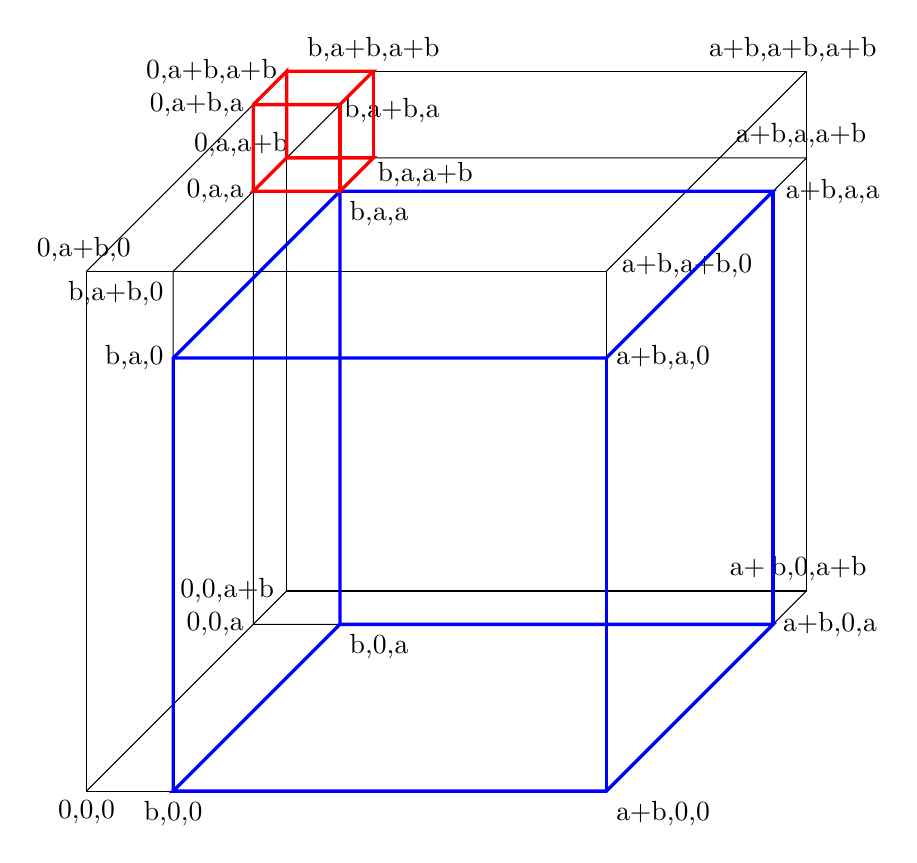
\begin{tikzpicture}[scale=1.1]

% Front face
\coordinate (A) at (0,0,0);
\node[below] at (A) {\sm{0,0,0}};
\coordinate (B) at (6,0,0);
\node[below right] at (B) {\sm{a+b,0,0}};
\coordinate (C) at (6,6,0);
\node[above right,xshift=2pt,yshift=-6pt] at (C)
  {\sm{a+b,a+b,0}};
\coordinate (D) at (0,6,0);
\node[above,xshift=-1pt] at (D) {\sm{0,a+b,0}};

% Front face
\coordinate (FF1) at (1,0,0);
\node[below] at (FF1) {\sm{b,0,0}};
\coordinate (FF2) at (1,5,0);
\node[left] at (FF2) {\sm{b,a,0}};
\coordinate (FF3) at (1,6,0);
\node[below left] at (FF3) {\sm{b,a+b,0}};
\coordinate (FF4) at (6,5,0);
\node[right] at (FF4) {\sm{a+b,a,0}};

% Back face
\coordinate (A1) at (0,0,-6);
\node[left,xshift=-1pt] at (A1) {\sm{0,0,a+b}};
\coordinate (B1) at (6,0,-6);
\node[above,xshift=-3pt] at (B1) {\sm{a+\:b,0,a+b}};
\coordinate (C1) at (6,6,-6);
\node[above,xshift=-5pt] at (C1) {\sm{a+b,a+b,a+b}};
\coordinate (D1) at (0,6,-6);
\node[left] at (D1) {\sm{0,a+b,a+b}};

% Back face
\coordinate (BF1) at (0,5,-6);
\node[above left,xshift=4pt,yshift=-3pt] at (BF1) 
  {\sm{0,a,a+b}};
\coordinate (BF2) at (1,5,-6);
\node[below right,xshift=-2pt,yshift=2pt] at (BF2)
  {\sm{b,a,a+b}};
\coordinate (BF3) at (1,6,-6);
\node[above] at (BF3) {\sm{b,a+b,a+b}};
\coordinate (BF4) at (6,5,-6);
\node[above,xshift=-2pt] at (BF4) {\sm{a+b,a,a+b}};

% Right face
\coordinate (RF1) at (6,5,-5);
\node[right,xshift=1pt] at (RF1) {\sm{a+b,a,a}};
\coordinate (RF2) at (6,0,-5);
\node[right] at (RF2) {\sm{a+b,0,a}};

% Bottom face
\coordinate (BT1) at (1,0,-5);
\node[below right] at (BT1) {\sm{b,0,a}};

% Left face
\coordinate (LF1) at (0,0,-5);
\node[left] at (LF1) {\sm{0,0,a}};
\coordinate (LF2) at (0,5,-5);
\node[left] at (LF2) {\sm{0,a,a}};
\coordinate (LF3) at (0,6,-5);
\node[left] at (LF3) {\sm{0,a+b,a}};

% Top face
\coordinate (TF1) at (1,6,-5);
\node[right,xshift=-2pt,yshift=-2pt] at (TF1) {\sm{b,a+b,a}};

% Internal point
\coordinate (I) at (1,5,-5);
\node[below right] at (I) {\sm{b,a,a}};


\draw (A) -- (B) -- (C) -- (D) -- cycle;
\draw (A1) -- (B1) -- (C1) -- (D1) -- cycle;
\draw (A) -- (A1);
\draw (B) -- (B1);
\draw (C) -- (C1);
\draw (D) -- (D1);

\draw (FF1) -- (FF2) -- (FF3) -- (BF3);
\draw (BF2) -- (FF2) -- (FF4) -- (BF4);
\draw (FF1) -- (BT1) -- (TF1);
\draw (BF3) -- (BF2);
\draw (TF1) -- (LF3);
\draw (LF3) -- (LF1) -- (RF2) -- (RF1) -- (LF2) -- 
      (BF1) -- (BF4);

\draw[very thick,blue] (FF1) -- (B) -- (RF2) -- (BT1) -- cycle; 
\draw[very thick,blue] (FF1) -- (FF2) -- (I) -- (BT1);
\draw[very thick,blue] (I) -- (RF1) -- (FF4) -- (FF2);
\draw[very thick,blue] (FF4) -- (B);
\draw[very thick,blue] (RF1) -- (RF2);

\draw[very thick,red] (I) -- (LF2) -- (BF1) -- (BF2) -- cycle;
\draw[very thick,red] (LF2) -- (LF3) -- (D1) -- (BF1);
\draw[very thick,red] (D1) -- (BF3) -- (TF1) -- (LF3);
\draw[very thick,red] (TF1) -- (I);
\draw[very thick,red] (BF3) -- (BF2);

\end{tikzpicture}
%\includegraphics[width=\textwidth]{Fig7_4}
\caption{$(a+b)^3=(a^3+b^3)+\cdots$}
\label{f.cardano1}
\end{figure}

%%%%%%%%%%%%%%%%%%%%%%%%%%%%%%%%%%%%%%%%%%%%%%%%%%%%%%%%%%%%%

\begin{figure}[htb]
\centering
\begin{tikzpicture}[scale=1.1]

% Front face
\coordinate (A) at (0,0,0);
\node[below] at (A) {\sm{0,0,0}};
\coordinate (B) at (6,0,0);
\node[below right] at (B) {\sm{a+b,0,0}};
\coordinate (C) at (6,6,0);
\node[above right,xshift=2pt,yshift=-6pt] at (C)
  {\sm{a+b,a+b,0}};
\coordinate (D) at (0,6,0);
\node[above,xshift=-1pt] at (D) {\sm{0,a+b,0}};

% Front face
\coordinate (FF1) at (1,0,0);
\node[below] at (FF1) {\sm{b,0,0}};
\coordinate (FF2) at (1,5,0);
\node[left] at (FF2) {\sm{b,a,0}};
\coordinate (FF3) at (1,6,0);
\node[below left] at (FF3) {\sm{b,a+b,0}};
\coordinate (FF4) at (6,5,0);
\node[right] at (FF4) {\sm{a+b,a,0}};

% Back face
\coordinate (A1) at (0,0,-6);
\node[left,xshift=-1pt] at (A1) {\sm{0,0,a+b}};
\coordinate (B1) at (6,0,-6);
\node[above,xshift=-3pt] at (B1) {\sm{a+\:b,0,a+b}};
\coordinate (C1) at (6,6,-6);
\node[above,xshift=-5pt] at (C1) {\sm{a+b,a+b,a+b}};
\coordinate (D1) at (0,6,-6);
\node[left] at (D1) {\sm{0,a+b,a+b}};

% Back face
\coordinate (BF1) at (0,5,-6);
\node[above left,xshift=4pt,yshift=-3pt] at (BF1) 
  {\sm{0,a,a+b}};
\coordinate (BF2) at (1,5,-6);
\node[below right,xshift=-2pt,yshift=2pt] at (BF2)
  {\sm{b,a,a+b}};
\coordinate (BF3) at (1,6,-6);
\node[above] at (BF3) {\sm{b,a+b,a+b}};
\coordinate (BF4) at (6,5,-6);
\node[above,xshift=-2pt] at (BF4) {\sm{a+b,a,a+b}};

% Right face
\coordinate (RF1) at (6,5,-5);
\node[right,xshift=1pt] at (RF1) {\sm{a+b,a,a}};
\coordinate (RF2) at (6,0,-5);
\node[right] at (RF2) {\sm{a+b,0,a}};

% Bottom face
\coordinate (BT1) at (1,0,-5);
\node[below right] at (BT1) {\sm{b,0,a}};

% Left face
\coordinate (LF1) at (0,0,-5);
\node[left] at (LF1) {\sm{0,0,a}};
\coordinate (LF2) at (0,5,-5);
\node[left] at (LF2) {\sm{0,a,a}};
\coordinate (LF3) at (0,6,-5);
\node[left] at (LF3) {\sm{0,a+b,a}};

% Top face
\coordinate (TF1) at (1,6,-5);
\node[right,xshift=-2pt,yshift=-2pt] at (TF1) {\sm{b,a+b,a}};

% Internal point
\coordinate (I) at (1,5,-5);
\node[below right] at (I) {\sm{b,a,a}};


\draw (A) -- (B) -- (C) -- (D) -- cycle;
\draw (A1) -- (B1) -- (C1) -- (D1) -- cycle;
\draw (A) -- (A1);
\draw (B) -- (B1);
\draw (C) -- (C1);
\draw (D) -- (D1);

\draw (FF1) -- (FF2) -- (FF3) -- (BF3);
\draw (BF2) -- (FF2) -- (FF4) -- (BF4);
\draw (FF1) -- (BT1) -- (TF1);
\draw (BF3) -- (BF2);
\draw (TF1) -- (LF3);
\draw (LF3) -- (LF1) -- (RF2) -- (RF1) -- (LF2) -- 
      (BF1) -- (BF4);

\draw[very thick,blue] (A) -- (FF1) -- (FF3) -- (D) -- cycle;
\draw[very thick,blue] (FF1) -- (BT1) -- (TF1) -- (FF3);
\draw[very thick,blue] (TF1) -- (LF3) -- (D);
\draw[very thick,blue] (LF3) -- (LF1) -- (A);
\draw[very thick,blue] (LF1) -- (BT1);

\draw[very thick,red] (LF1) -- (RF2) -- (RF1) -- (LF2);
\draw[very thick,red] ($(LF2) + (2pt,0)$) -- ($(LF1) + (2pt,0)$);
\draw[very thick,red] (A1) -- (B1) -- (BF4) -- (BF1) -- cycle;
\draw[very thick,red] ($(LF2) + (2pt,0)$) -- ($(BF1) + (2pt,0)$);
\draw[very thick,red] (BF4) -- (RF1);
\draw[very thick,red] (B1) -- (RF2);
\draw[very thick,red] (A1) -- (LF1);

\draw[very thick,green] (FF2) -- (FF4) -- (C) -- (FF3);
\draw[very thick,green] 
  ($(FF2) + (2pt,0)$) -- ($(FF3) + (2pt,0)$);
\draw[very thick,green] 
  ($(FF4) + (0,2pt)$) -- ($(BF4) + (0,2pt)$);
\draw[very thick,green] (BF4) -- (C1) -- (BF3);
\draw[very thick,green] 
  ($(BF3) + (2pt,0)$) -- ($(FF3) + (2pt,0)$);
\draw[very thick,green] (C1) -- (C);
\draw[very thick,green] (BF3) -- (BF2) -- (FF2);
\draw[very thick,green] 
  ($(BF2) + (0,2pt)$) -- ($(BF4) + (0,2pt)$);


\end{tikzpicture}
%\includegraphics[width=\textwidth]{Fig7_5}
\caption{$(a+b)^3=\cdots+3ab(a+b)$}\label{f.cardano2}
\end{figure}

\section{Les nombres imaginaires ne les intimidaient pas}\label{s.imaginary}

L'histoire des mathématiques montre une progression des concepts qui étaient initialement considérés comme dénués de sens, mais qui ont finalement été compris, acceptés et se sont avérés utiles. De toute évidence, puisque les nombres comptent des choses, $-1$, un nombre négatif, n'a pas de sens. Il est évident que puisque les nombres sont des rapports d'entiers (nombres rationnels), $\sqrt{2}$, dont on peut facilement prouver qu'il est irrationnel, n'a pas de sens. De toute évidence, $\sqrt{-1}$, la racine carrée d'un nombre négatif, n'a aucun sens puisqu'il n'existe aucun nombre --- entier, rationnel ou réel --- dont le carré est égal à $-1$.

La compréhension complète des racines carrées des nombres négatifs, encore appelés aujourd'hui nombres imaginaires  bien qu'ils ne soient pas moins réels que les nombres réels, n'a pas été atteinte avant le XIX$^\text{e}$ siècle. Il est donc surprenant que, dès le XVI$^\text{e}$ siècle, Jérôme Cardan et Raphaël Bombelli  aient refusé de se laisser intimider par ce concept et aient fait les premiers pas vers la compréhension de ces nombres.

Considérons l'équation du second degré :
\begin{align}
x^2-10x+40=0\,.\label{eq.cardano-quadratic}
\end{align}
Par la formule bien connue (équation~\ref{eq.quadratic-roots}),
\[
r_1, r_2=\displaystyle\frac{10\pm\sqrt{100-160}}{2}=5\pm\sqrt{-15}\,.
\]
Nous ne savons rien des racines carrées des nombres négatifs et nous ne savons pas quelles sont ces valeurs, mais comme Cardan nous savons d'après le théorème~\ref{eq.quadratic-roots} que 
\begin{align*}
r_1+r_2&=(5+\sqrt{-15})+(5-\sqrt{-15})=10=-b\\
r_1r_2&=(5+\sqrt{-15})(5-\sqrt{-15})=25-5\sqrt{-15}+5\sqrt{-15}-(-15)=40=c,
\end{align*}
qui correspondent aux coefficients de l'équation du second degré (\ref{eq.cardano-quadratic}). Il est assez intuitif que $\sqrt{-15}+(-\sqrt{-15})=0$ même si nous ne savons rien de $\sqrt{-15}$, et de même, il est assez intuitif que $\sqrt{-15}\cdot-(\sqrt{-15})=-(-15)=15$ même si nous ne savons pas ce qu'est $\sqrt{-15}$.

\enlargethispage{\baselineskip}

Considérons maintenant l'équation de degré trois
\begin{align}
x^3-15x-4=0\,.\label{eq.bombelli-cubic}
\end{align}
Il n'est pas difficile d'observer que 4 est une racine, mais comment l'obtenir? La formule de Cardan donne la racine 
\begin{align}
r=\sqrt[3]{2+11\sqrt{-1}}+\sqrt[3]{2-11\sqrt{-1}}\,,\label{eq.cube-root}
\end{align}
une formule assez compliquée qui n'a aucun rapport évident avec 4. 

Bombelli a courageusement effectué le calcul suivant (voir l'équation~\ref{eq.car}):
\begin{align*}
(2+\sqrt{-1})^3&=
8+3\cdot 4\sqrt{-1}+3\cdot 2(-1)+(-1\sqrt{-1})=
2+11\sqrt{-1}\\
(2-\sqrt{-1})^3&=
8-3\cdot 4\sqrt{-1}+3\cdot 2(-1)-(-1\sqrt{-1})=
2-11\sqrt{-1}\,.
\end{align*}
D'après l'équation~\ref{eq.cube-root},
\begin{align*}
r&=\sqrt[3]{2+11\sqrt{-1}} + \sqrt[3]{2-11\sqrt{-1}}\\
&=\sqrt[3]{(2+\sqrt{-1})^3} + \sqrt[3]{(2-\sqrt{-1})^3}\\
&=(2+\sqrt{-1}) + (2-\sqrt{-1})=4\,.
\end{align*}


%%%%%%%%%%%%%%%%%%%%%%%%%%%%%%%%%%%%%%%%%%%%%%%%%%%%%%%%

\section{La méthode de Lill et le cercle de Carlyle}\label{s.lill-quadratic}

On peut appliquer la méthode de Lill pour résoudre les équations du second degré.\footnote{Cette section suppose que vous avez lu la méthode de Lill dans le chapitre~\ref{c.origami-cube}.} A titre d'exemple, nous utilisons l'équation~\ref{eq.quadratic-lill} qui donne les racines d'une équation du second degré obtenue par factorisation :
\[
x^2+bx+c=x^2-4x+3= (x-1)(x-3)\,.
\]
En appliquant la méthode de Lill, on obtient les chemins de  la figure~\ref{f.lill-quadratic}.

\begin{figure}[htbp]
\centering
\begin{tikzpicture}[scale=1.1]
% Draw help lines and axes
\draw[step=10mm,white!50!black] (-4,-5) grid (2,1);
\draw[thick] (-4,0) -- (2,0);
\draw[thick] (0,-5) -- (0,1);
\foreach \x in {-3,...,2}
  \node at (\x-.2,.2) {\sm{\x}};
\foreach \y in {-4,...,-1}
  \node at (-.2,\y-.3) {\sm{\y}};

 Draw first path
\coordinate (A) at (0,0);
\coordinate (B) at (1,0);
\coordinate (C) at (1,-4);
\coordinate (D) at (-2,-4);
\draw[very thick] (A) --
  node[above] {$1$} (B);
\draw[very thick,name path=bc] (B) -- 
  node[right,xshift=-1pt,yshift=6pt] {$b=-4$} (C);
\draw[very thick,name path=cd] (C) --
  node[below left,xshift=3pt] {$c=3$}(D);

% Draw first segment of second path
\path[name path=a2] (A) -- +(-45:1.414);
\path [name intersections = {of = a2 and bc, by = {A2}}];
\node[above right] at (A2) {$P_1$};
\draw[very thick,dashed] (A) -- (A2);
\draw ($(A) + (14pt,0)$)
  arc [start angle=0, end angle = -45, radius=14pt];
\node[below right,xshift=40pt,yshift=-2pt] at (A) {$-45^\circ$};
\draw[->] ($(A)+(33pt,-6pt)$) -- +(-18pt,0);
\draw[rotate=135] (A2) rectangle +(5pt,5pt);

% Draw second segment of second path
\path[name path=b2] (A2) -- +(-135:5);
\path [name intersections = {of = b2 and cd, by = {B2}}];
\draw[very thick,dashed] (A2) -- (B2);

% Draw first segment of second path
\path[name path=a3] (A) -- +(-71.57:4);
\path [name intersections = {of = a3 and bc, by = {A3}}];
\node[above right] at (A3) {$P_2$};
\draw[very thick,dashed] (A) -- (A3);
\draw ($(A) + (20pt,0)$)
  arc [start angle=0, end angle = -71.57, radius=20pt];
\node[below right,xshift=40pt,yshift=-10pt] at (A) {$-\mbox{71,57}^\circ$};
\draw[->] ($(A)+(35pt,-13pt)$) -- +(-18pt,0);
\draw[rotate=108.43] (A3) rectangle +(5pt,5pt);

% Draw second segment of second path
\path[name path=b3] (A3) -- +(198.43:5);
\path [name intersections = {of = b3 and cd, by = {B3}}];
\draw[very thick,dashed] (A3) -- (B3);

\end{tikzpicture}
%\includegraphics[width=0.8\textwidth]{Fig7_6}
\caption{La méthode de Lill pour $x^2-4x+3$.}\label{f.lill-quadratic}
\end{figure}
Vérifions que les angles sont corrects:
\[
-\tan (-45^\circ) = -1,\quad -\tan (-\mbox{71,57}^\circ) \approx -3\,.
\]
Pour les équations du second degré, on peut trouver les points $P_1$ et $P_2$ comme  intersections de la droite représentant le coefficient $b$ et du cercle dont le diamètre est la droite reliant le point de départ et le point d'arrivée des chemins (fig.~\ref{f.lill-circle}). Pour qu'un point de la droite $b$ soit une racine, la réflexion de la droite doit être $90^\circ$ et donc l'angle inscrit est sous-tendu par un diamètre.

\begin{figure}[htbp]
\centering
\begin{tikzpicture}[scale=1]
% Draw help lines and axes
\draw[step=10mm,white!50!black] (-4,-5) grid (2,1);
\draw[thick] (-4,0) -- (2,0);
\draw[thick] (0,-5) -- (0,1);
\foreach \x in {-3,...,2}
  \node at (\x-.2,.2) {\sm{\x}};
\foreach \y in {-4,...,-1}
  \node at (-.2,\y-.3) {\sm{\y}};

 Draw first path
\coordinate (A) at (0,0);
\coordinate (B) at (1,0);
\coordinate (C) at (1,-4);
\coordinate (D) at (-2,-4);
\draw[very thick] (A) --
  node[above] {$1$} (B);
\draw[very thick,name path=bc] (B) -- 
  node[right,xshift=-2pt,yshift=6pt] {$b=-4$} (C);
\draw[very thick,name path=cd] (C) --
  node[below left,xshift=-1pt,yshift=-5pt] {$c=3$}(D);

% Draw first segment of second path
\path[name path=a2] (A) -- +(-45:1.414);
\path [name intersections = {of = a2 and bc, by = {A2}}];
\node[above right] at (A2) {$P_1$};
\draw[dashed] (A) -- (A2);
\draw ($(A) + (14pt,0)$)
  arc [start angle=0, end angle = -45, radius=14pt];
\node[below right,xshift=40pt,yshift=-2pt] at (A) {$-45^\circ$};
\draw[->] ($(A)+(33pt,-6pt)$) -- +(-18pt,0);
\draw[rotate=135] (A2) rectangle +(5pt,5pt);

% Draw second segment of second path
\path[name path=b2] (A2) -- +(-135:5);
\path [name intersections = {of = b2 and cd, by = {B2}}];
\draw[dashed] (A2) -- (B2);

% Draw first segment of second path
\path[name path=a3] (A) -- +(-71.57:4);
\path [name intersections = {of = a3 and bc, by = {A3}}];
\node[above right] at (A3) {$P_2$};
\draw[dashed] (A) -- (A3);
\draw ($(A) + (20pt,0)$)
  arc [start angle=0, end angle = -71.57, radius=20pt];
\node[below right,xshift=40pt,yshift=-10pt] at (A) {$-\mbox{71,57}^\circ$};
\draw[->] ($(A)+(35pt,-13pt)$) -- +(-18pt,0);
\draw[rotate=108.43] (A3) rectangle +(5pt,5pt);

% Draw second segment of second path
\path[name path=b3] (A3) -- +(198.43:5);
\path [name intersections = {of = b3 and cd, by = {B3}}];
\draw[dashed] (A3) -- (B3);

\coordinate (O) at (-1,-2);
\vertex{O};
\node[draw,circle through=(A)] at (O) {};
\draw[very thick,dotted] (A) -- (D);

\end{tikzpicture}
%\includegraphics[width=0.8\textwidth]{Fig7_7}
\caption{Construction d'un cercle pour trouver les racines.}\label{f.lill-circle}
\end{figure}

Ceci peut également être vérifié par le calcul. Le centre du cercle est le milieu du diamètre $(-1,-2)$. La longueur du diamètre est 
\[
\sqrt{(-2)^2+(-4)^2}=\sqrt{20}\,,
\]
donc le carré de la longueur du rayon est $\left(\sqrt{20/2}\right)^2=5$. Nous avons besoin de l'intersection de ce cercle et de la droite $x=1$ :
\begin{align*}
(x-(-1))^2+(y-(-2))^2&=r^2\\
(x^2+2x+1)+(y^2+4y+4)&=5\\
y^2+4y+3&=0\\
y&=-1,\;-3\,.
\end{align*}


Une méthode similaire pour résoudre les équations du second degré est le cercle de Carlyle, antérieur à la méthode de Lill. Étant donné une équation du second degré $x^2-bx+c$ (notons le signe moins du terme linéaire), construisons des points en $(0,1)$ et $(b,c)$. Construisons un cercle dont le diamètre est le segment reliant les deux points (fig.~\ref{f.carlyle-circle}). Ses intersections (s'il y en a) avec l'axe des $x$ sont les racines de l'équation.

Dans le cas général, le centre du cercle est $(b/2,(c-(-1))/2)$ et la longueur du diamètre est $\sqrt{b^2+(c-1)^2}$, donc l'équation du cercle est :
\[
\left(x-\frac{b}{2}\right)^2+\left(y-\frac{c+1}{2}\right)^2=
\frac{b^2+(c-1)^2}{4}\,.
\]
Pour l'exemple, en substituant $b=4,c=3$ et $y=0$, on voit que $x=1$ et $x=3$ sont les racines de l'équation du second degré.


\begin{figure}[htbp]
\centering
\begin{tikzpicture}[scale=1]
% Draw help lines and axes
\draw[step=10mm,white!50!black] (-1,-1) grid (5,5);
\draw[thick] (-1,0) -- (5,0);
\draw[thick] (0,-1) -- (0,5);
\foreach \x in {0,...,5}
  \node at (\x-.2,.2) {\sm{\x}};
\foreach \y in {1,...,4}
  \node at (-.1,\y+.2) {\sm{\y}};

\coordinate (A) at (0,1);
\node[below left] at (A) {$(0,1)$};
\coordinate (B) at (4,3);
\node[above right] at (B) {$(4,3)$};
\vertex{A};
\vertex{B};

\coordinate (O) at (2,2);
\vertex{O};
\node[draw,circle through=(B)] at (O) {};
\draw[very thick,dotted] (A) -- (B);

\coordinate (X1) at (1,0);
\node[below left] at (X1) {$(1,0)$};
\coordinate (X2) at (3,0);
\node[below right] at (X2) {$(3,0)$};
\vertex{X1};
\vertex{X2};

\end{tikzpicture}
%\includegraphics[width=0.8\textwidth]{Fig7_8}
\caption{Cercle de Carlyle pour $x^2-4x+3$.}\label{f.carlyle-circle}
\end{figure}


\section{Calcul numérique des racines}\label{s.numerical}


Les élèves apprennent le calcul symbolique des racines, des dérivées, etc. Aujourd'hui, la plupart des calculs sont effectués par des ordinateurs et le calcul symbolique est donc moins important. L'analyse numérique est la branche des mathématiques et de l'informatique qui développe des méthodes de calcul précises et efficaces. Le principal défi consiste à gérer la finitude des valeurs stockées dans la mémoire de l'ordinateur. Le calcul 
\[\mbox{0,12}\times \mbox{0,14}=\mbox{0,0168}\]
est facile à faire, mais 
\[
\mbox{0,123456789}\times \mbox{0,123456789}\]
nécessite dix-huit chiffres pour être représenté avec précision, ce qui n'est pas possible dans une mémoire qui contient seize chiffres. Cette erreur s'appelle une \emph{erreur d'arrondi}.

Un problème encore plus sérieux se produit  lorsqu'on utilise l'arithmétique à virgule flottante. De toute évidence,
\[(\mbox{0,12}\times 10^{-10})\times (\mbox{0,14}\times 10^{-8})\]
ne serait pas calculé en écrivant tous les zéros. Au lieu de cela, nous multiplions les mantisses et additionnons les exposants pour obtenir $\mbox{0,0168}\times 10^{-18}$, qui est normalisé en $\mbox{0,168}\times 10^{-19}$ de sorte que le chiffre le plus significatif apparaisse après la virgule, assurant ainsi une précision maximale étant donné la taille fixe de la mantisse. Si l'exposant maximal pouvant être représenté est de $-16$, le résultat ne peut tout simplement pas être stocké. Cette erreur est appelée \emph{soupassement en virgule flottante}.



La formule pour trouver les racines de l'équation du second degré $x^2+bx+c$ est 
\begin{align}
r_1, r_2 = \frac{-b\pm\sqrt{b^2-4c}}{2}\,.\label{eq.quadratic-numerical}
\end{align}
Considérons ce qui se passe si $b=1000$ et $c=4$. Les racines sont 
\[
r_1, r_2 = \frac{-1000\pm\sqrt{1\,000\,000-16}}{2}\,.
\]
Selon la précision de l'arithmétique, il est possible qu'une des racines soit si proche de zéro que la valeur stockée soit nulle. L'évaluation de l'équation du second degré donne le résultat surprenant $0^2+b\cdot 0 +4= 4= 0$.

Peut-on faire mieux? D'après l'équation~\ref{eq.viete-quad},
\[
r_1+r_2 = -b\,,\quad\quad r_1r_2=c\,.
\]
Si $r_2$ est très inférieur à $r_1$, ce qui s'écrit $r_2\ll r_1$, alors $r_1\approx -b$ et $r_2\approx -c/b$. Le tableau~\ref{t.quadratic}, obtenu par un programme informatique, compare les valeurs des racines calculées par ces formules avec les valeurs obtenues par la formule traditionnelle (équation~\ref{eq.quadratic-numerical}). On fixe la valeur de $c$  à 4 et on représente les racines pour des valeurs croissantes de $b$.

Initialement, les valeurs réelles calculées par la formule traditionnelle pour $r_2$ sont plus précises ($r_2-r_{2v}$ est négatif) mais à partir de $b=100\,000$, le calcul basé sur l'équation~\ref{eq.viete-quad} est plus précis. Telles sont les surprises de l'analyse numérique.

\begin{table}[htbp]
\footnotesize
\caption{Deux calculs des racines d'une équation du second degré. $r_1$ et $r_2$ sont les racines calculées par l'équation~\ref{eq.quadratic-numerical}. $r_{1v}$ et $r_{2v}$ sont les racines calculées par l'équation~\ref{eq.viete-quad}. Les erreurs sont $r_{i}-r_{iv}$. Les valeurs sont tronquées à quatre décimales.
On écrit les nombres à virgule flottante sous la forme $4e-5$ au lieu de $4\times 10^{-5}$ car les programmes informatiques sont normalement écrits sous forme de suites linéaires de caractères.} \label{t.quadratic}
\[
\begin{array}{r@{\hspace{2mm}}r@{\hspace{2mm}}r@{\hspace{2mm}}r@{\hspace{2mm}}r@{\hspace{2mm}}r@{\hspace{2mm}}r}
\hline
\noalign{\smallskip}
b & r_1 & r_{1v} & \mathrm{erreur}_1 & r_2 & r_{2v} & \mathrm{erreur}_2\\
\noalign{\smallskip}\hline\noalign{\smallskip}
100  &  -\mbox{99,9599}  &  -100  &  \mbox{0,0400}  &  -\mbox{0,04001}\  &  -\mbox{0,04}  &  -\mbox{1,6012}e\!-\!05\\
1000  &  -\mbox{999,9959}  &  -1000  &  \mbox{0,0040}  &  -\mbox{0,0040}  &  -\mbox{0,004}  &  -\mbox{1,6000}e\!-\!08\\
10000  &  -\mbox{9999,9996}  &  -10000  &  \mbox{0,0004}  &  -\mbox{0,0004}  &  -\mbox{0,0004}  &  -\mbox{1,6270}e\!-\!11\\
100000  &  -\mbox{99999,9999}  &  -100000  &  \mbox{3,9999}e\!-\!5  &  -\mbox{3,9999}e\!-\!5  &  -4e\!-\!5  &  \mbox{1,0104}e\!-\!12\\
1000000  &  -\mbox{999999,9999}  &  -1000000  &  \mbox{4,0000}e\!-\!6  &  -\mbox{3,9999}e\!-\!6  &  -4e\!-\!6  &  \mbox{2,7749}e\!-\!11\\
10000000  &  -\mbox{10000000,0}  &  -10000000  &  \mbox{3,9860}e\!-\!7  &  -\mbox{3,9953}e\!-\!7  &  -4e\!-\!7  &  \mbox{4,6261}e\!-\!10\\
 \noalign{\smallskip}
 \hline
\end{array}
\]
\end{table}


\subsection*{Quelle est la surprise ?}

L'approche de Poh-Shen Loh fournit une nouvelle façon de voir la relation entre les coefficients et les racines que l'on ne voit pas simplement en mémorisant la formule traditionnelle. Ce qui est surprenant, c'est que cette relation est fondamentale dans la démonstration algébrique de Gauss de la constructibilité d'un heptadécagone régulier (chap.~\ref{c.heptadecagon}).

Avec la prédominance moderne des méthodes algébriques en géométrie, il est important de rappeler que l'inverse était autrefois vrai. Comme le montrent les constructions d'Al-Khwârizmî et de Cardan, les méthodes géométriques étaient utilisées pour obtenir des résultats en algèbre. Lill et Carlyle ont tous deux développé des méthodes géométriques pour résoudre des équations du second degré. Les considérations sur le calcul numérique sur ordinateur surprendront les étudiants qui n'y ont pas encore été confrontés.

\subsection*{Sources}
La méthode de Poh-Shen Loh est issue de \cite{loh1,loh2}. La construction d'Al-Khwârizmî provient de \cite[chapitre~1]{jorg} et \cite{mastin}. La construction de Cardan se trouve dans \cite[chap.~1]{jorg}. Pour l'histoire pittoresque  de la formule de Cardan, voir \cite{wiki:cardano}. \cite[chapitre~2]{jorg} présente les premières tentatives de calcul avec des nombres imaginaires. La méthode de Lill et le cercle de Carlyle se trouvent dans \cite{wiki:quadratic}, ainsi qu'une discussion sur le calcul numérique des racines.
